\documentclass{standalone}
\usepackage{tikz}
\usetikzlibrary{patterns, positioning}
\usepackage[sfdefault]{ClearSans} %% option 'sfdefault' activates Clear Sans as the default text font
\usepackage[T1]{fontenc}

\begin{document}
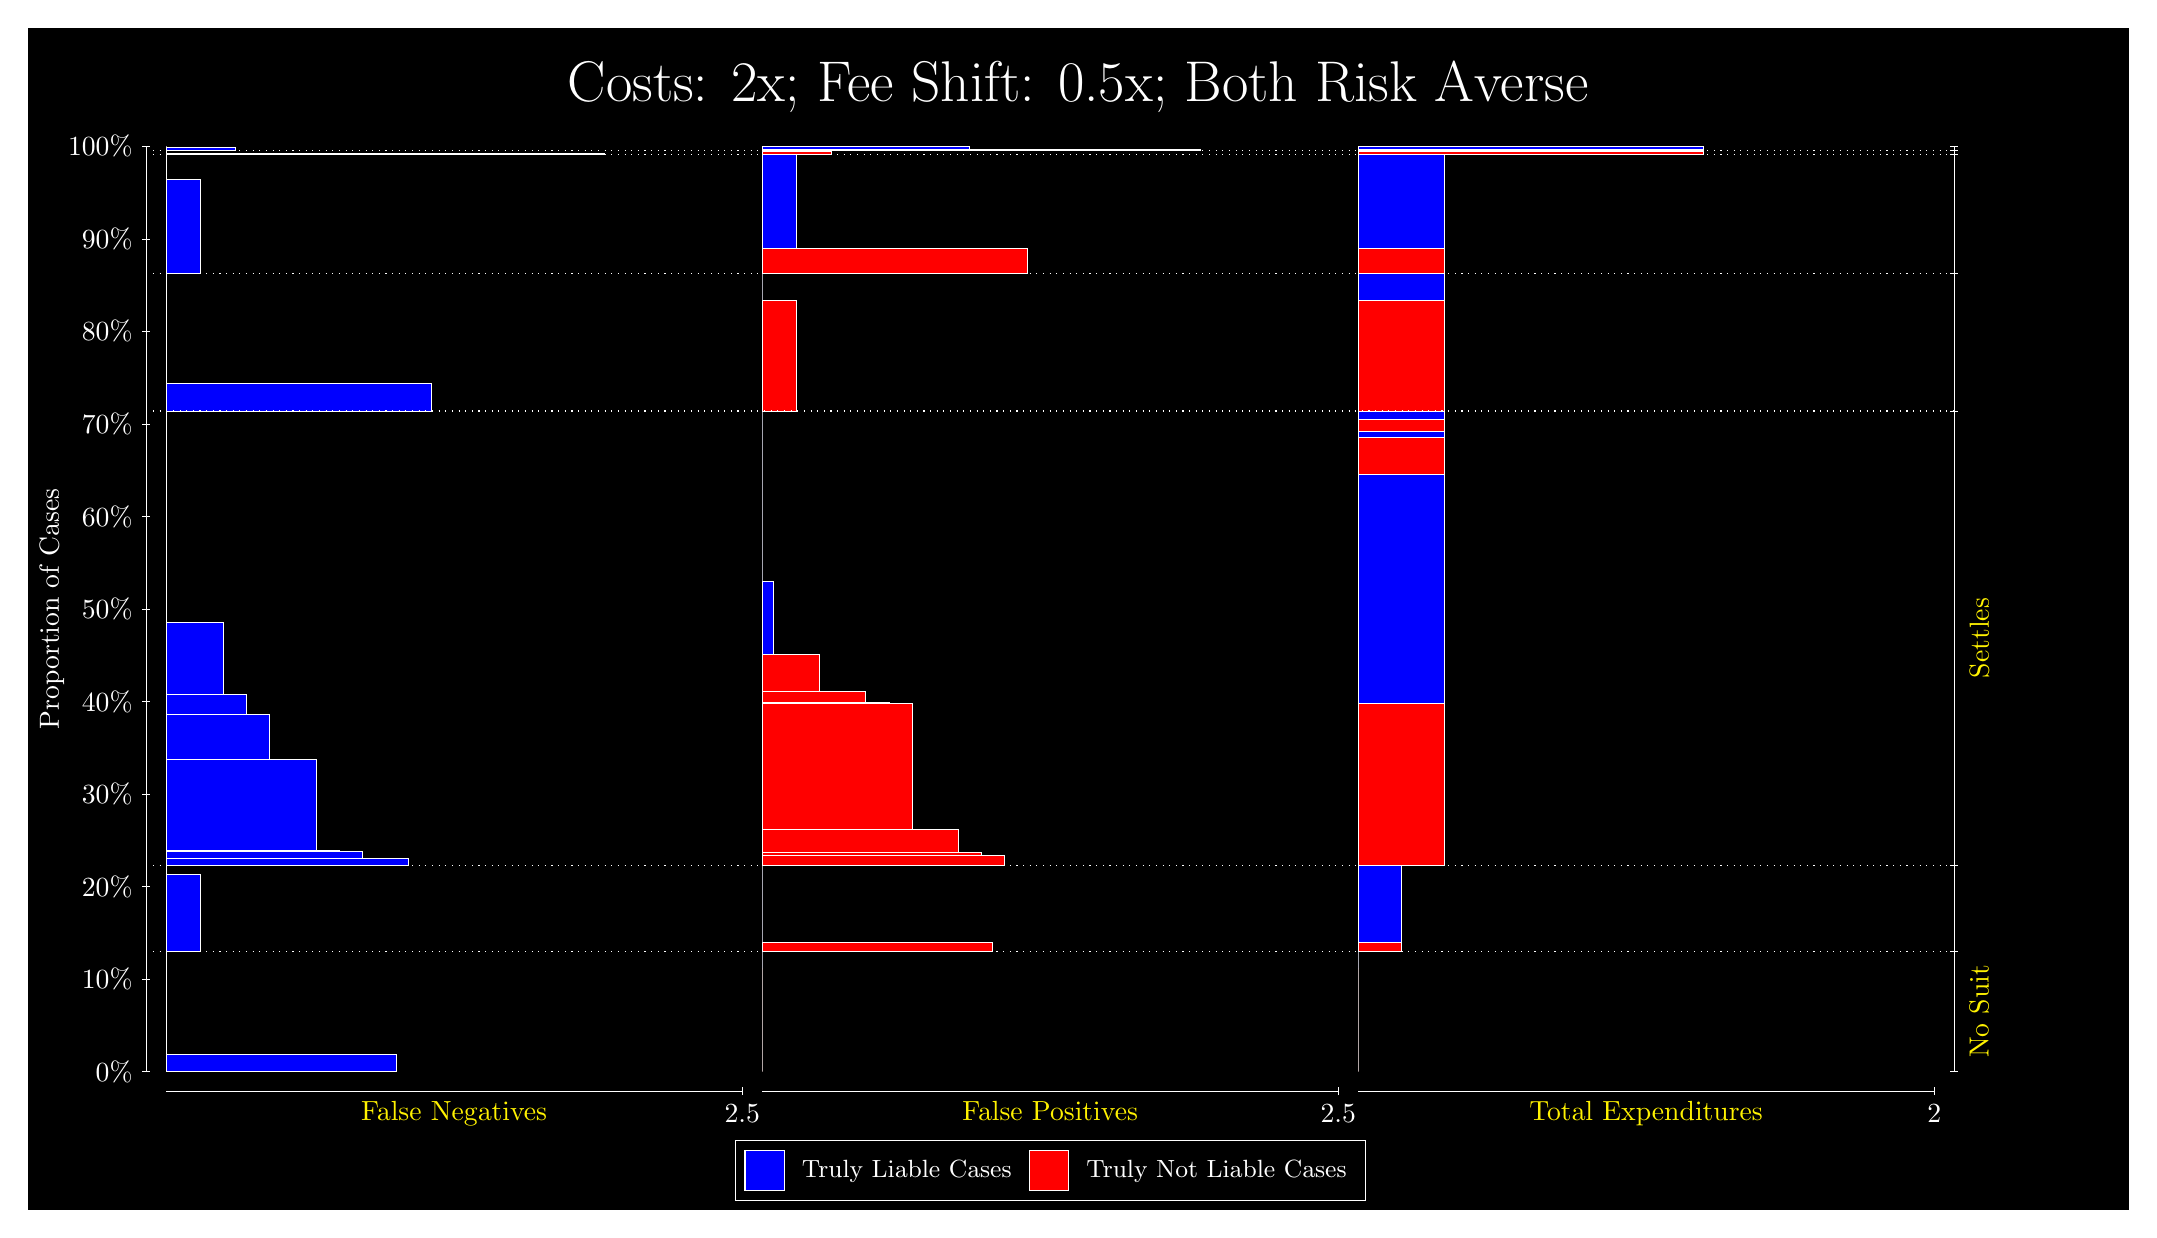
\begin{tikzpicture}
\draw[fill=black] (0,0) rectangle (26.667,15);
\draw[text=white] (0,13.5) rectangle (26.667,15) node[midway] {\huge Costs: 2x; Fee Shift: 0.5x; Both Risk Averse};
\draw[white, very thin] (1.5,1.75) -- (1.5,13.5);
\node[rotate=90, text=white, anchor=center] at (0.3, 7.625) {Proportion of Cases};
\draw[white, very thin] (1.45,1.75) -- (1.55,1.75);
\node[text=white, anchor=east] at (1.45, 1.75) {0\%};
\draw[white, very thin] (1.45,2.925) -- (1.55,2.925);
\node[text=white, anchor=east] at (1.45, 2.925) {10\%};
\draw[white, very thin] (1.45,4.1) -- (1.55,4.1);
\node[text=white, anchor=east] at (1.45, 4.1) {20\%};
\draw[white, very thin] (1.45,5.275) -- (1.55,5.275);
\node[text=white, anchor=east] at (1.45, 5.275) {30\%};
\draw[white, very thin] (1.45,6.45) -- (1.55,6.45);
\node[text=white, anchor=east] at (1.45, 6.45) {40\%};
\draw[white, very thin] (1.45,7.625) -- (1.55,7.625);
\node[text=white, anchor=east] at (1.45, 7.625) {50\%};
\draw[white, very thin] (1.45,8.8) -- (1.55,8.8);
\node[text=white, anchor=east] at (1.45, 8.8) {60\%};
\draw[white, very thin] (1.45,9.975) -- (1.55,9.975);
\node[text=white, anchor=east] at (1.45, 9.975) {70\%};
\draw[white, very thin] (1.45,11.15) -- (1.55,11.15);
\node[text=white, anchor=east] at (1.45, 11.15) {80\%};
\draw[white, very thin] (1.45,12.325) -- (1.55,12.325);
\node[text=white, anchor=east] at (1.45, 12.325) {90\%};
\draw[white, very thin] (1.45,13.5) -- (1.55,13.5);
\node[text=white, anchor=east] at (1.45, 13.5) {100\%};

\draw[white, very thin] (24.457,1.75) -- (24.457,13.5);
\draw[white, very thin] (24.407,1.75) -- (24.507,1.75);
\node[anchor=west] at (24.407, 1.75) {};
\draw[white, very thin] (24.407,3.2791) -- (24.507,3.2791);
\node[anchor=west] at (24.407, 3.2791) {};
\draw[white, very thin] (24.407,4.3722) -- (24.507,4.3722);
\node[anchor=west] at (24.407, 4.3722) {};
\draw[white, very thin] (24.407,10.139) -- (24.507,10.139);
\node[anchor=west] at (24.407, 10.139) {};
\draw[white, very thin] (24.407,11.89) -- (24.507,11.89);
\node[anchor=west] at (24.407, 11.89) {};
\draw[white, very thin] (24.407,13.398) -- (24.507,13.398);
\node[anchor=west] at (24.407, 13.398) {};
\draw[white, very thin] (24.407,13.449) -- (24.507,13.449);
\node[anchor=west] at (24.407, 13.449) {};
\draw[white, very thin] (24.407,13.5) -- (24.507,13.5);
\node[anchor=west] at (24.407, 13.5) {};

\draw[white, very thin, fill=blue] (1.75,1.75) rectangle (4.6775,1.9656);
\draw[white, very thin, fill=red] (1.75,1.9656) rectangle (1.75,3.2791);
\draw[white, very thin, fill=blue] (1.75,3.2791) rectangle (2.1891,4.2572);
\draw[white, very thin, fill=red] (1.75,4.2572) rectangle (1.75,4.3722);
\draw[white, very thin, fill=blue] (1.75,4.3722) rectangle (4.8239,4.4527);
\draw[white, very thin, fill=blue] (1.75,4.4527) rectangle (4.2384,4.5416);
\draw[white, very thin, fill=blue] (1.75,4.5416) rectangle (3.9457,4.5551);
\draw[white, very thin, fill=blue] (1.75,4.5551) rectangle (3.6529,5.7104);
\draw[white, very thin, fill=blue] (1.75,5.7104) rectangle (3.0674,6.2933);
\draw[white, very thin, fill=blue] (1.75,6.2933) rectangle (2.7746,6.5379);
\draw[white, very thin, fill=blue] (1.75,6.5379) rectangle (2.4819,7.4611);
\draw[white, very thin, fill=red] (1.75,7.4611) rectangle (1.75,10.139);
\draw[white, very thin, fill=blue] (1.75,10.139) rectangle (5.1167,10.486);
\draw[white, very thin, fill=red] (1.75,10.486) rectangle (1.75,11.89);
\draw[white, very thin, fill=blue] (1.75,11.89) rectangle (2.1891,13.084);
\draw[white, very thin, fill=red] (1.75,13.084) rectangle (1.75,13.398);
\draw[white, very thin, fill=blue] (1.75,13.398) rectangle (7.3123,13.415);
\draw[white, very thin, fill=red] (1.75,13.415) rectangle (1.75,13.449);
\draw[white, very thin, fill=blue] (1.75,13.449) rectangle (2.6283,13.483);
\draw[white, very thin, fill=red] (1.75,13.483) rectangle (1.75,13.5);
\draw[white, very thin, fill=red] (9.3189,1.75) rectangle (9.3189,3.0635);
\draw[white, very thin, fill=blue] (9.3189,3.0635) rectangle (9.3189,3.2791);
\draw[white, very thin, fill=red] (9.3189,3.2791) rectangle (12.246,3.3941);
\draw[white, very thin, fill=blue] (9.3189,3.3941) rectangle (9.3189,4.3722);
\draw[white, very thin, fill=red] (9.3189,4.3722) rectangle (12.393,4.4977);
\draw[white, very thin, fill=red] (9.3189,4.4977) rectangle (12.1,4.5311);
\draw[white, very thin, fill=red] (9.3189,4.5311) rectangle (11.807,4.8251);
\draw[white, very thin, fill=red] (9.3189,4.8251) rectangle (11.222,6.4272);
\draw[white, very thin, fill=red] (9.3189,6.4272) rectangle (10.929,6.4454);
\draw[white, very thin, fill=red] (9.3189,6.4454) rectangle (10.636,6.5776);
\draw[white, very thin, fill=red] (9.3189,6.5776) rectangle (10.051,7.0497);
\draw[white, very thin, fill=blue] (9.3189,7.0497) rectangle (9.4652,7.9728);
\draw[white, very thin, fill=blue] (9.3189,7.9728) rectangle (9.3189,10.139);
\draw[white, very thin, fill=red] (9.3189,10.139) rectangle (9.758,11.542);
\draw[white, very thin, fill=blue] (9.3189,11.542) rectangle (9.3189,11.89);
\draw[white, very thin, fill=red] (9.3189,11.89) rectangle (12.686,12.205);
\draw[white, very thin, fill=blue] (9.3189,12.205) rectangle (9.758,13.398);
\draw[white, very thin, fill=red] (9.3189,13.398) rectangle (10.197,13.432);
\draw[white, very thin, fill=blue] (9.3189,13.432) rectangle (9.3189,13.449);
\draw[white, very thin, fill=red] (9.3189,13.449) rectangle (14.881,13.466);
\draw[white, very thin, fill=blue] (9.3189,13.466) rectangle (11.954,13.5);
\draw[white, very thin, fill=red] (16.888,1.75) rectangle (16.888,3.0635);
\draw[white, very thin, fill=blue] (16.888,3.0635) rectangle (16.888,3.2791);
\draw[white, very thin, fill=red] (16.888,3.2791) rectangle (17.437,3.3941);
\draw[white, very thin, fill=blue] (16.888,3.3941) rectangle (17.437,4.3722);
\draw[white, very thin, fill=red] (16.888,4.3722) rectangle (17.986,6.4272);
\draw[white, very thin, fill=blue] (16.888,6.4272) rectangle (17.986,9.3332);
\draw[white, very thin, fill=red] (16.888,9.3332) rectangle (17.986,9.8053);
\draw[white, very thin, fill=blue] (16.888,9.8053) rectangle (17.986,9.8857);
\draw[white, very thin, fill=red] (16.888,9.8857) rectangle (17.986,10.036);
\draw[white, very thin, fill=blue] (16.888,10.036) rectangle (17.986,10.139);
\draw[white, very thin, fill=red] (16.888,10.139) rectangle (17.986,11.542);
\draw[white, very thin, fill=blue] (16.888,11.542) rectangle (17.986,11.89);
\draw[white, very thin, fill=red] (16.888,11.89) rectangle (17.986,12.205);
\draw[white, very thin, fill=blue] (16.888,12.205) rectangle (17.986,13.398);
\draw[white, very thin, fill=red] (16.888,13.398) rectangle (21.279,13.432);
\draw[white, very thin, fill=blue] (16.888,13.432) rectangle (21.279,13.449);
\draw[white, very thin, fill=red] (16.888,13.449) rectangle (21.279,13.466);
\draw[white, very thin, fill=blue] (16.888,13.466) rectangle (21.279,13.5);
\draw[white, dotted] (1.5,3.2791) -- (24.457,3.2791);
\draw[white, dotted] (1.5,4.3722) -- (24.457,4.3722);
\draw[white, dotted] (1.5,10.139) -- (24.457,10.139);
\draw[white, dotted] (1.5,11.89) -- (24.457,11.89);
\draw[white, dotted] (1.5,13.398) -- (24.457,13.398);
\draw[white, dotted] (1.5,13.449) -- (24.457,13.449);
\draw[white, very thin] (1.75,1.5) -- (9.0689,1.5);
\node[text=yellow, anchor=north] at (5.4094, 1.5) {False Negatives};
\draw[white, very thin] (9.0689,1.45) -- (9.0689,1.55);
\node[text=white, anchor=north] at (9.0689, 1.45) {2.5};

\draw[white, very thin] (9.3189,1.5) -- (16.638,1.5);
\node[text=yellow, anchor=north] at (12.978, 1.5) {False Positives};
\draw[white, very thin] (16.638,1.45) -- (16.638,1.55);
\node[text=white, anchor=north] at (16.638, 1.45) {2.5};

\draw[white, very thin] (16.888,1.5) -- (24.207,1.5);
\node[text=yellow, anchor=north] at (20.547, 1.5) {Total Expenditures};
\draw[white, very thin] (24.207,1.45) -- (24.207,1.55);
\node[text=white, anchor=north] at (24.207, 1.45) {2};

\node[text=yellow, centered, rotate=90] at (24.777, 2.5146) {No Suit};

\node[text=yellow, centered, rotate=90] at (24.777, 7.2554) {Settles};





\draw (12.978300999999998,1.5) node[draw=none] (baseCoordinate) {};
\begin{scope}[align=center]
        \matrix[scale=0.5, draw=white, below=0.5cm of baseCoordinate, nodes={draw}, column sep=0.1cm]{
            \node[rectangle, draw, minimum width=0.5cm, minimum height=0.5cm, fill=blue] {}; &
            \node[draw=none, font=\small, text=white] (B) {Truly Liable Cases}; &
            \node[rectangle, draw, minimum width=0.5cm, minimum height=0.5cm, fill=red] {}; &
            \node[draw=none, font=\small, text=white] (B) {Truly Not Liable Cases}; \\
            };
\end{scope}

\end{tikzpicture}
\end{document}